%%%
%%%     xDNCL言語マニュアル (グラフィック拡張編)
%%%
%%% 初版
%%% 2008/09/22 - 11:10 by H.Toyoda
%%%
\documentclass[11pt,a4j]{jarticle}
%\pagestyle{empty}
\usepackage{amsmath}
\usepackage{amssymb}
\usepackage{epsfig}
\usepackage{color}
%\usepackage{txfonts}

\setlength{\topmargin}{-20mm}
\setlength{\oddsidemargin}{-15mm}
\setlength{\textheight}{255mm}
\setlength{\textwidth}{185mm}

%---------- 箇条書き -----------

\newenvironment{itemize2}%  
{%
   \begin{list}{$\bullet$\ \ }% 見出し記号/直後の空白を調節
   {%
      \setlength{\itemindent}{0pt}
      \setlength{\leftmargin}{3zw}%  左のインデント
      \setlength{\rightmargin}{0zw}% 右のインデント
      \setlength{\labelsep}{0zw}%    黒丸と説明文の間
      \setlength{\labelwidth}{3zw}%  ラベルの幅
      \setlength{\itemsep}{0em}%     項目ごとの改行幅
      \setlength{\parsep}{0em}%      段落での改行幅
      \setlength{\listparindent}{0zw}% 段落での一字下り
   }
}{%
   \end{list}%
}
%---------- 番号つき箇条書き -----------

\newcounter{enum2}
\newenvironment{enumerate2}{%
   \begin{list}%
   {%
      \arabic{enum2}.\ \,%  見出し記号/直後の空白を調節
   }%
   {%
      \usecounter{enum2}
      \setlength{\itemindent}{0zw}%  ここは 0 に固定
      \setlength{\leftmargin}{3zw}%  左のインデント
      \setlength{\rightmargin}{0zw}% 右のインデント
      \setlength{\labelsep}{0zw}%    黒丸と説明文の間
      \setlength{\labelwidth}{3zw}%  ラベルの幅
      \setlength{\itemsep}{0em}%     項目ごとの改行幅
      \setlength{\parsep}{0em}%      段落での改行幅
      \setlength{\listparindent}{0zw}% 段落での一字下り
   }
}{%
   \end{list}%
}
\setlength{\topsep}{0pt}
\setlength{\itemsep}{10pt}
\setlength{\parsep}{0mm}
\setlength{\itemindent}{50mm}

%\labelsep 20mm
%\labelwidth 50mm
%\leftmargin 100mm
\newcommand{\ExerciseTitle}[1]{%
  \begin{center}\Large
    \textbf{PEN マニュアル Q \& A} \qquad \texttt{#1}
  \end{center}%
}

\renewcommand{\baselinestretch}{1.0}

\begin{document}

%\ExerciseTitle{22nd\_April\_2006}
%\begin{flushright}
%{\small	2008/10/14}
%\end{flushright}
\begin{center}
\begin{LARGE}
{\bf{(補足)~グラフ描画のための関数群\\
\ \\}}
\end{LARGE}
\end{center}

 このドキュメントは、PENの描画機能を用いて、主として2次元座標
平面上でグラフを描画するためのものである。
描画ウィンドウを開くためにはgOpenWindow()の代わりに
gOpenGraphWindow()関数を用いる。
これによって、2次元仮想平面上の任意の矩形領域を描画ウィンドウに
マッピングすることができる。
以後の描画命令は、仮想平面に対して『図形描画のための関数群』を
そのまま利用することができる。

gSetMap()関数は、仮想平面上の原点の並行移動もしくは、仮想平面上
の任意の矩形領域を描画ウィンドウに再マッピングするためのものである。

%  グラフ描画のための関数は以下の関数群から構成される。
%\begin{itemize2}
%  \item [(1)] 描画のためのウィンドウのオープン/クローズ関数 
%  \item [(2)] 図形の属性を指定するための関数 
%  \item [(3)] 図形を描画するための関数 
%\end{itemize2}
%
%  図形は、一つのウィンドウ上に描画する。このウィンドウの大きさを指定し
%て開くための関数として gOpenGraphWindow()がある。 gCloseWindow()は閉じるた
%めの関数であるが、この関数を呼び出すと描画ウィンドウが画面から消滅す
%るので、通常gCloseWindow()を使用することはない。 \\
%  図形は、線分、折れ線などの{\bf{線図形}}、長方形、楕円、
%多角形などの{\bf{面図形}}、
%および、{\bf{文字図形}}からなる。 図形を描くには、原則として先に描画属性を指 
%定しなければな らない。描画属性としては、線の太さ、線の種類、線の色等 
%の線図形に適応されるもの、塗りつぶしの色等の面図形に適応されるもの、 
%および、フォントの種類、フォントサイズ等の文字図形に適応されるものが 
%ある。描画属性を指定しない場合は、予め定められた属性値が用いられ、一 
%旦、設定した属性値は、同じ属性に対して新たに設定されるまで有効である。 
%  図形を描画するための関数としてここでは、多角形の描画の関数を示す。 \\
%
%  以下、各関数について説明する。

%(1) グラフ描画のためのウィンドウのオープン/クローズ関数 
グラフ描画のためのウィンドウのオープン/クローズ関数 

\begin{enumerate2}
\item {\bf{gOpenGraphWindow(実数 width, 実数 height, 実数 x1, 実数 y1, 実数 x2, 実数 y2, 論理値 axis)}} \\
%   \ \ 実数  width, height, x1, x2, y1, y2  \\
%   \ \ 論理値 axis
\vspace{-5mm}
   \begin{quotation}
   幅 width、高さ height の描画ウィンドウを開く。
   ウィンドウの左下を(x1,y1)座標とし、右上を(x2, y2)座標
   となるような座標平面として定義する。
   axis の値を true, false に指定することで座標軸の表示、非表示を指定する。
   \end{quotation}
   \begin{quotation}
\begin{figure}[!h]
\begin{center}
\begin{minipage}{24zw}
	   \noindent $[$使用例$]$\\
\ \\
幅500、高さ500の描画ウィンドウを用意し、
そのウィンドウの左下を(-100,-50)、右上を(350,300)の仮想座標空間として定義する。
また、xy座標軸を表記する。(図~\ref{fig:gopengraphwindow}) \\

{\small{gOpenGraphWindow(500, 500, -50, 350, -100, 300, true)}}
\end{minipage}
\begin{minipage}{20zw}
%\begin{figure}[!h]
\begin{center}
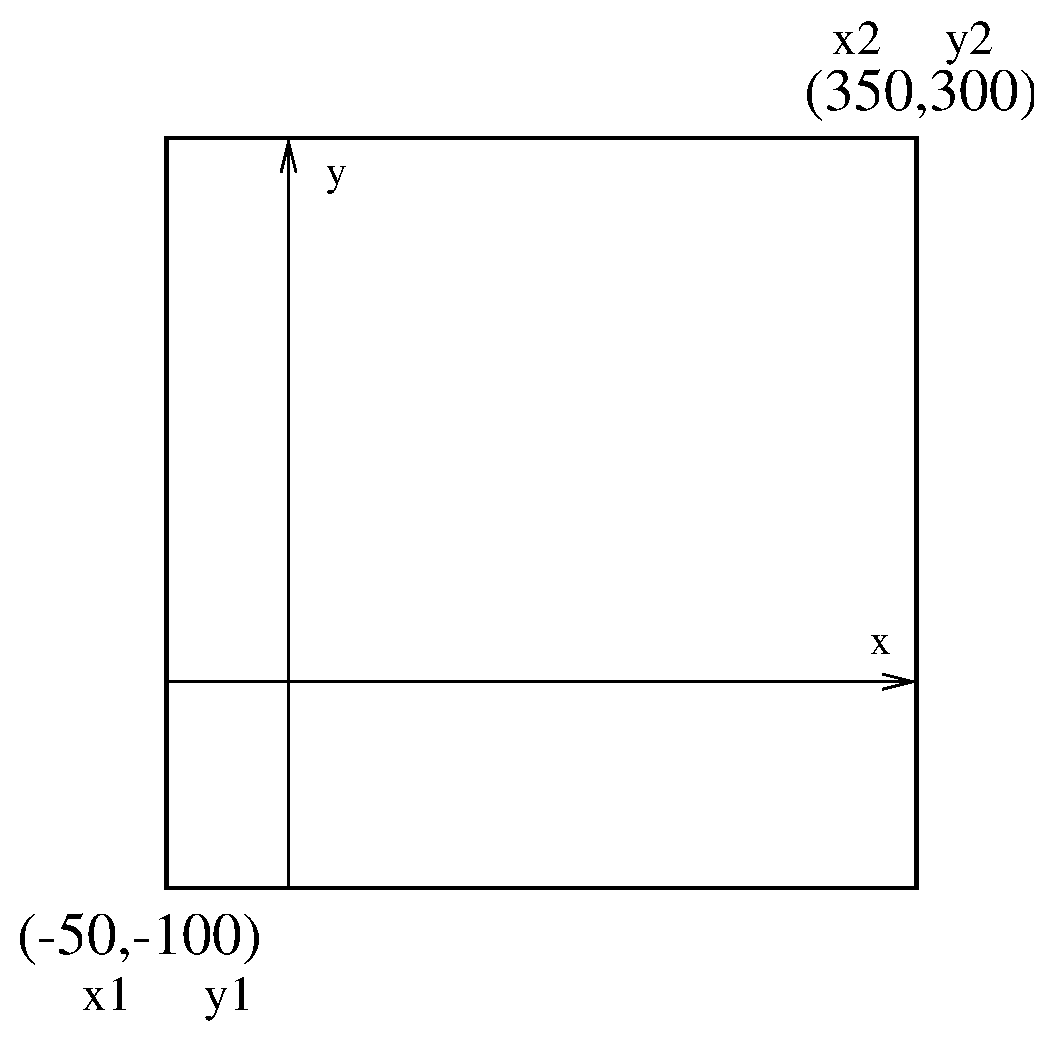
\epsfig{file=./eps/gopengraphwindow.eps, width=1.9in}
\caption{$\!\!\!\!$\colorbox{white}{{\textcolor{white}{:}}}}
%\caption{gOpenGraphWindowの例}
\label{fig:gopengraphwindow}
\end{center}
%\end{figure}
\end{minipage}
\end{center}
\end{figure}
   \end{quotation}


\item {\bf{gSetMap(実数x1, 実数y1, 実数x2, 実数y2)}} \\
%  \ \    実数 x1, x2, y1, y2
  \begin{quotation}
     描画ウィンドウの左下を点(x1,y1)、右上を点(x2,y2)として再指定する。
     (図~\ref{fig:gsetmaps02})\\
  \end{quotation}
\begin{quotation}
\begin{figure}[!h]
\begin{minipage}{25zw}
\noindent $[$使用例$]$ \\

図~\ref{fig:gopengraphwindow}のウィンドウを開いた後、
左下を(0,50)、右上を(50,200)の座標空間として再定義する。\\


{\small{
 gOpenGraphWindow(500, 500, -50, 350, -100, 300, true)
 gSetMap(0, 200, -50, 150) \\
}}
\end{minipage}
\begin{minipage}{20zw}
%\begin{figure}[!h]
\begin{center}
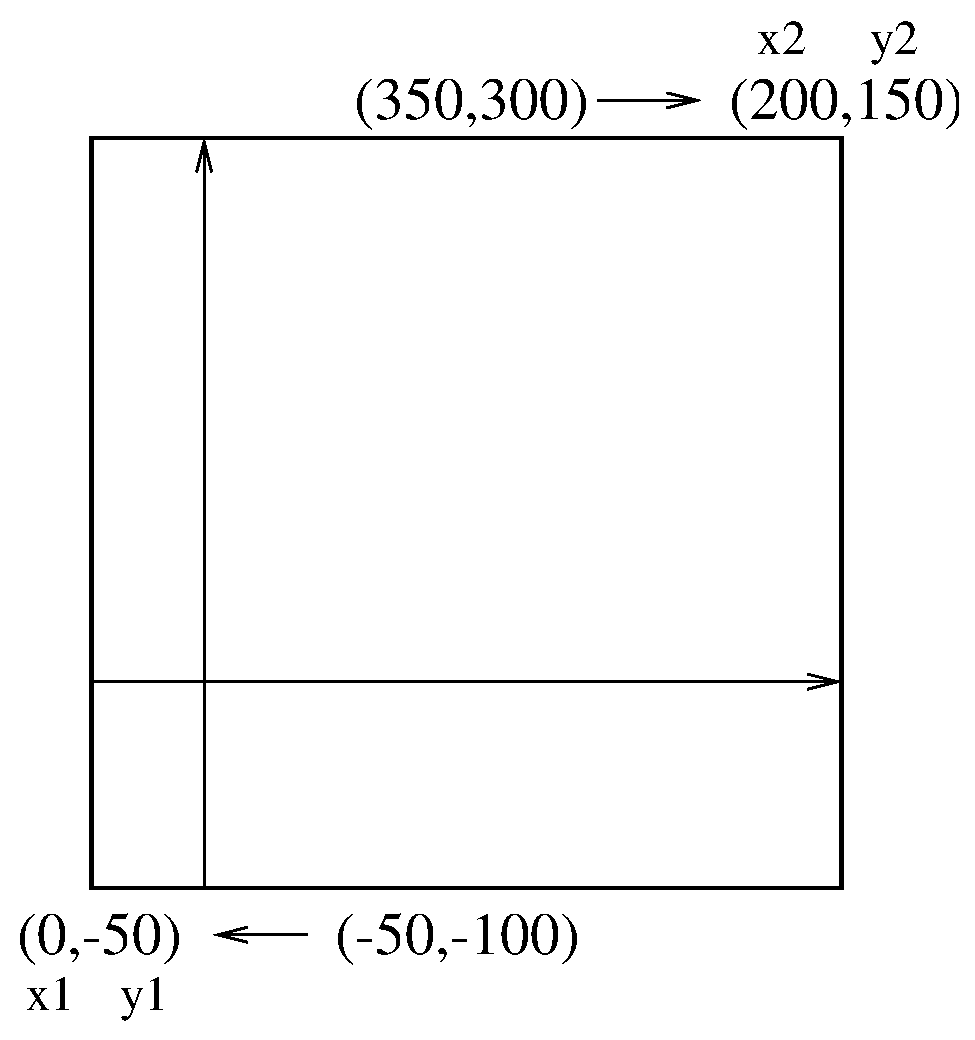
\epsfig{file=./eps/gsetmaps02.eps, width=2.0in}
\caption{$\!\!\!\!$\colorbox{white}{{\textcolor{white}{:}}}}
\label{fig:gsetmaps02}
\end{center}
%\end{figure}
\end{minipage}
\end{figure}
   \end{quotation}
\end{enumerate2}

\end{document}

%%%xDNCL-draw.tex へ移動
%%% gSetMap --> gSetOrigin へ名称変更(の予定)
%%%
\item {\bf{gSetMap(実数x, 実数y)}} \\
%   \ \  実数 x, y 
\vspace{-5mm}
   \begin{quotation}
     描画ウィンドウの左上からの右方向にx、下方向にyの点を原点として再定義する。
   \end{quotation}
   \begin{quotation}
\begin{figure}[!h]
\begin{center}
\begin{minipage}{25zw}
	   \noindent $[$使用例$]$\\

\noindent 図~\ref{fig:gopengraphwindow}の描画ウィンドウの
(100,150)を中心とする円(r=50)を描いた後に、この座標空間の(100,0)を原点に再定義する。
そして、再定義した原点を中心とする円(r=50)を描く。(図~\ref{fig:gsetmaps01})
\ \\

{\small{
          gOpenGraphWindow(500, 500, -50, 350, -100, 300, true)
          gSetLineColor(255, 0, 0)  \\
          gDrawCircle(100, 150, 50)  \\
          gSetMap(150, 300) \\
          gSetLineColor(0, 255, 0)  \\
          gDrawCircle(0, 0, 50)  \\
}}
\end{minipage}
\begin{minipage}{20zw}
%\begin{figure}[!h]
\begin{center}
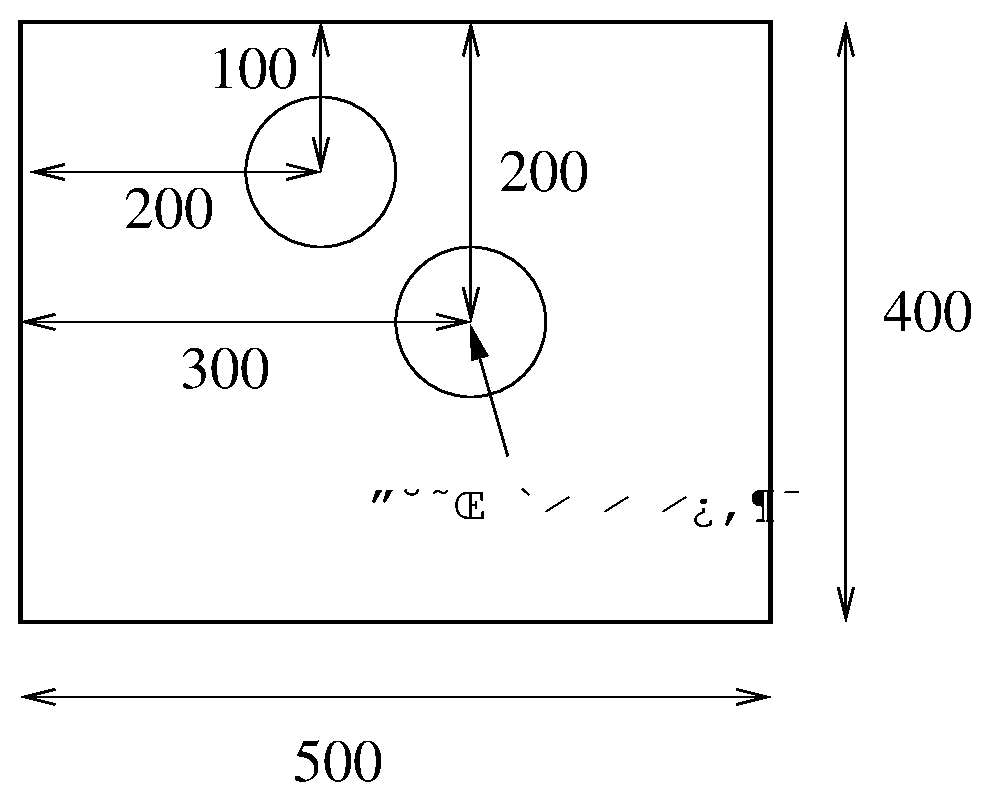
\epsfig{file=./eps/gsetmaps01.eps, width=2.0in}
\caption{$\!\!\!\!$\colorbox{white}{{\textcolor{white}{:}}}}
\label{fig:gsetmaps01}
\end{center}
%\end{figure}
\end{minipage}
\end{center}
\end{figure}
\end{quotation}


